%% ma: L12-B01-0033
%% lop: 12
%% chuong: 1
%% bai: 1
%% dang: 12.1.3
%% loai: TN4
%% muc: NB
%% dap_an: "C"
%% nguon: "HK1-DeOn_1_1.pdf (M10, Đề ôn tập học kì 1 Toán 12, Đề số 2), Phần I Câu 2"
%% kien_thuc: "Bài 1 (tính đơn điệu và cực trị)"
%% trang_thai: chinh-thuc
\begin{ex}
Cho hàm số $y=f(x)$ liên tục trên $\mathbb R$ và có bảng biến thiên như sau:
\begin{center}\begin{tikzpicture}
\tkzTabInit[lgt=1.2,espcl=2.4]{$x$/.8,$y'$/.8,$y$/2.2}{$-\infty$,$-2$,$1$,$+\infty$}
\tkzTabLine{,-,0,+,0,-,}
\tkzTabVar{+/$+\infty$,-/$-1$,+/$3$,-/$-\infty$}
\end{tikzpicture}\end{center}
Hàm số đã cho đồng biến trên khoảng nào dưới đây?
\choice{$(-\infty;-2)$}{$(-2;+\infty)$}{\True $(-2;0)$}{$(-\infty;1)$}
\loigiai{Hàm số đồng biến trên $(-2;1)$, nên đồng biến trên $(-2;0)\subset(-2;1)$.}
\end{ex}
